% Supplementary material: complete formulation of the bilevel siting model and its solution method.
% Build: pdflatex formulation; bibtex formulation; pdflatex formulation (x2).
\documentclass[11pt]{article}
\usepackage[margin=1in]{geometry}
\usepackage{cite}
\usepackage{amsmath,amssymb,amsfonts,amsthm}
\usepackage{graphicx,booktabs,array,xcolor,textcomp}
\usepackage[hyphens]{url}
\usepackage{tikz}
\usetikzlibrary{arrows.meta,positioning,fit,calc,backgrounds,shapes.misc}
\usepackage{algorithm}
\usepackage{algorithmic}
\usepackage[utf8]{inputenc}
\usepackage[hidelinks]{hyperref}
%% macros.tex -- shared macros for the ITSC paper (IEEEtran conference class).
\newif\ifanon \anontrue   % set to \anonfalse and fill in main.tex to show the authors
%% Units.
\newcommand{\usd}{~USD}
\newcommand{\pct}{\%}
%% Colour scheme shared by all figures and tables.
\definecolor{cOurs}{HTML}{2A78D6}    % layouts found by our method
\definecolor{cRule}{HTML}{EB6834}    % rule layouts (coverage, spread)
\definecolor{cPilot}{HTML}{E34948}   % DOT 2024 pilot
\definecolor{cRole}{HTML}{6250D6}    % role variants (swap-only cabinet, charging hub)
\definecolor{cGrey}{HTML}{9A9A9A}    % context
%% Figure inclusion that still builds while a figure file is missing.
%% #1 = file, #2 = width, #3 = placeholder height.
\newcommand{\figfile}[3]{\IfFileExists{#1}{\includegraphics[width=#2]{#1}}{\fbox{\parbox[c][#3][c]{\dimexpr#2-2\fboxsep-2\fboxrule\relax}{\centering\footnotesize missing: \texttt{\detokenize{#1}}}}}}

\newtheorem{proposition}{Proposition}
\renewcommand{\thesection}{\Roman{section}}
\renewcommand{\thesubsection}{\thesection-\Alph{subsection}}
\title{Supplementary Material: Complete Formulation\\[2pt]\large Battery-Swapping and Charging Stations for E-Bike Food Delivery in Manhattan}
\author{}
\date{}
\begin{document}
\maketitle
\noindent The paper describes the lower level and the bounds in words and keeps four equations. This supplement gives the complete formulation that the released code implements: the upper level (Section~\ref{sec:bilevel}), the lower-level integer program (Section~\ref{sec:model}) and the solution method with its bounds (Section~\ref{sec:method}). Section numbers ``of the paper'' refer to the main paper. Equation numbers here are those of this supplement.
\setcounter{section}{1}
\providecommand{\rSC}{\textsf{SC}}
\providecommand{\rS}{\textsf{S}}
\providecommand{\rC}{\textsf{C}}
\providecommand{\OPEX}{\mathrm{OPEX}}
\providecommand{\UB}{\mathrm{UB}}
\providecommand{\LB}{\mathrm{LB}}
\providecommand{\Vopen}{V^{\mathrm{open}}}
\providecommand{\Vall}{V^{\mathrm{all}}}

\section{Bilevel Model}\label{sec:setup}\label{sec:bilevel}

In this section, we state the bilevel model in full. Fig.~\ref{fig:bilevel} shows its two levels. The upper level is the city planner, who chooses a layout within a budget to minimize the set-up cost per day plus the expected operating cost. The lower level is the delivery operation. For each evening it assigns orders to riders, plans swaps, charging and transfers, and returns the operating cost. Both levels minimize the same cost, so for one to three budget units the two levels can also be written as one two-stage program (Section~\ref{sec:model:objective}). In the 15-site study a dispatch rule replaces the lower-level integer program (Section~\ref{sec:method:fifteen}).

\begin{figure}[t]
  \centering
  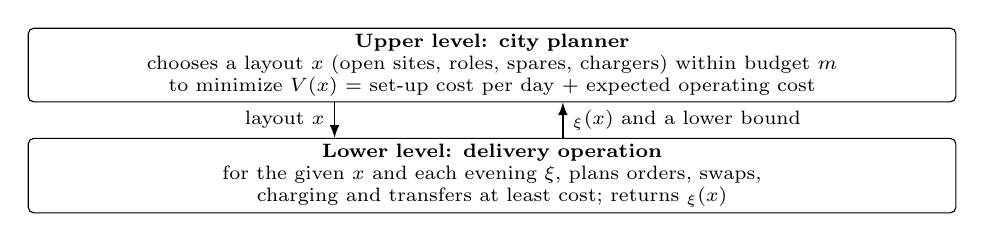
\begin{tikzpicture}[font=\scriptsize,
    lvl/.style={draw,rounded corners=2pt,align=center,inner sep=2pt,text width=0.96\columnwidth},
    arr/.style={-latex,line width=0.6pt}]
    \node[lvl] (up) {\textbf{Upper level: city planner}\\
      chooses a layout $x$ (open sites, roles, spares, chargers) within budget $m$\\
      to minimize $V(x)$ = set-up cost per day + expected operating cost};
    \node[lvl,below=0.45cm of up] (lo) {\textbf{Lower level: delivery operation}\\
      for the given $x$ and each evening $\xi$, plans orders, swaps, charging and transfers at least cost; returns $\OPEX_\xi(x)$};
    \draw[arr] ([xshift=-2cm]up.south) -- node[left]{layout $x$} ([xshift=-2cm]lo.north);
    \draw[arr] ([xshift=0.9cm]lo.north) -- node[right]{$\OPEX_\xi(x)$ and a lower bound} ([xshift=0.9cm]up.south);
  \end{tikzpicture}
  \caption{The planner (upper level) chooses a layout; the delivery operation (lower level) plans each evening for that layout and returns the operating cost. With its constraints relaxed, it also returns a lower bound (Section~\ref{sec:method}).}
  \label{fig:bilevel}
\end{figure}

\subsection{Upper Level: the Planner}\label{sec:model:upper}
We first state the planner's decision. The planner chooses among candidate locations ($\Lambda$; 59 in Manhattan), the candidate sites of the text. At an open location $l$ it builds one station with a role $\mu\in\{\rSC,\rS,\rC\}$. The pair $j=(l,\mu)$ is an \emph{object}, so each location has three possible objects, at most one open. A swap-and-charge site (\rSC; also called a full site) swaps and recharges batteries from one shared stock. A swap-only cabinet (\rS) hands out its spares but cannot recharge them. A charging-only hub (\rC) only recharges batteries brought to it. At each location the planner picks at most one option $\psi=(\mu_\psi,B_\psi,C_\psi)$ from a short menu $\Psi_l$. An option fixes the role and the numbers of spares and chargers. The menu offers $B\in\{2,3,4\}$ and $C\in\{1,2\}$ for a swap-and-charge site, $B\in\{2,3\}$ for a swap-only cabinet, and $C\in\{2,4\}$ for a hub. A hub holds no spares ($B_\psi=0$) and is offered only at the 12 hub-capable locations. The binary $w_{l\psi}$ is one if option $\psi$ is built at $l$. Let $\mathcal J$ be the set of all objects, $\mathcal S\subseteq\mathcal J$ the swap-capable ones (roles \rSC, \rS) and $\mathcal C\subseteq\mathcal J$ the charge-capable ones (roles \rSC, \rC). The planner's choice must satisfy
\begin{gather}
  \textstyle\sum_{\psi\in\Psi_l}w_{l\psi}\le1,\qquad l\in\Lambda,\label{eq:one-option}\\
  \textstyle (y_j,B_j,C_j)=\sum_{\psi\in\Psi_l:\,\mu_\psi=\mu}(1,B_\psi,C_\psi)\,w_{l\psi},\label{eq:maps}\\
  \textstyle\sum_{j\in\mathcal J}\big(\hat F y_j+\hat b B_j+\hat c C_j\big)\le 52{,}150\,m,\label{eq:budget}\\
  \textstyle\sum_{j\in\mathcal S}y_j\ge1,\qquad y_j\le\sum_{j'\in\mathcal C}y_{j'}\ \ (j\ \text{of role \rS}),\label{eq:admissible}
\end{gather}
where row \eqref{eq:one-option} allows at most one option per location. Row \eqref{eq:maps} reads off the chosen option for every object $j=(l,\mu)$: $y_j$ is one if the object is open, $B_j$ is its number of full spares at the start of the evening and $C_j$ its number of chargers. The menu respects each site's storage cap $K_j=8$ batteries and charger cap $\bar C_j=4$, and a hub has $C_j\ge y_j$. Row \eqref{eq:budget} keeps the investment within $m$ budget units, with $\hat F=50{,}000$, $\hat b=450$ and $\hat c=400$\usd{} per site, spare battery and charger. One swap-and-charge site with three spares and two chargers costs exactly one unit. The budget caps how many sites open, not which. Row \eqref{eq:admissible} requires at least one swap-capable object, since every rider must end the evening within reach of an open swap site. For every swap-only cabinet it also requires a charge-capable partner in the layout. The partner need not be within transfer range, because a cabinet can also run on its spares alone. A \emph{layout} is $x=(y,B,C)$; $\mathcal X_m$ is the set of layouts that satisfy \eqref{eq:one-option}--\eqref{eq:admissible}.



\paragraph*{Scenarios and the planner's cost}\label{sec:model:objective}
A scenario ($\xi\in\Xi$) is one 16:00--20:00 evening, the dinner peak, with its orders and the riders' start positions and charge levels. The $|\Xi|=12$ scenarios have weights $p_\xi$ (5/42 on weekdays, 2/42 at weekends). The set-up cost of an evening is a quarter of the day's fixed cost, since the evening covers 4 of 16 operating hours. The day's fixed cost is the yearly cost spread over 360 days:
\begin{equation}\label{eq:setup}
  \mathrm{setup}(x)=\textstyle\sum_{j\in\mathcal J}\big(F_jy_j+b^BB_j+b^CC_j\big),
\end{equation}
with $F_j=12.03$ per site (29.19 for a hub), $b^B=0.332$ per spare and $b^C=0.082$ per charger, all in USD. The yearly cost repays the investment at 7\pct{} over 10 years (site), 3 years (spare) and 5 years (charger). It also includes running costs: 10,200 per year for a site (rent, insurance, maintenance) and 5\pct{} of a charger's price per year. A spare also pays for one full charge each evening (0.6~kWh at the charging efficiency 0.9 of Section~\ref{sec:model}, so 0.67~kWh), at the flat rate of 0.32\usd{} per kWh. A hub is priced on 100,000\usd{} of investment and 27,800 per year of running cost, so 29.19 per day. The budget \eqref{eq:budget} still counts it at 50,000, as one site. A standard site (three spares, two chargers) then costs 13.19\usd{} per evening. Throughout the paper, ``per day'' means this per-evening cost. The planner's cost adds the weighted operating cost of the 12 evenings:
\begin{equation}\label{eq:siting}
  \begin{gathered}
  V(x)=\mathrm{setup}(x)+\textstyle\sum_{\xi\in\Xi}p_\xi\,\OPEX_\xi(x),\\
  \OPEX_\xi(x)=\min\big\{\mathbf c^\top\boldsymbol\zeta:\ \boldsymbol\zeta\in\mathcal Z_\xi(x)\big\},
  \end{gathered}
\end{equation}
where $\OPEX_\xi(x)$, the operating cost of an evening, is the optimum of the lower level (Section~\ref{sec:model}). Its variables $\boldsymbol\zeta$ range over $\mathcal Z_\xi(x)$, the set of integer points that satisfy \eqref{eq:flow}--\eqref{eq:endtargets} and the transfer rows of Section~\ref{sec:model} for layout $x$, and $\mathbf c$ is the cost vector of \eqref{eq:opex}. If $\mathcal Z_\xi(x)$ is empty, $\OPEX_\xi(x)=+\infty$. The planner's optimum at budget $m$ is $V^*_m=\min_{x\in\mathcal X_m}V(x)$. In bilevel form (Fig.~\ref{fig:bilevel}), the lower-level plan is an optimal response to the layout:
\begin{equation}\label{eq:bilevel}
  \begin{gathered}
  \min_{x\in\mathcal X_m}\ \mathrm{setup}(x)+\textstyle\sum_{\xi}p_\xi\,\mathbf c^\top\boldsymbol\zeta_\xi\\
  \text{s.t.}\ \ \boldsymbol\zeta_\xi\in\arg\min\{\mathbf c^\top\boldsymbol\zeta:\ \boldsymbol\zeta\in\mathcal Z_\xi(x)\},\ \ \xi\in\Xi.
  \end{gathered}
\end{equation}
Therefore, \eqref{eq:bilevel} has the same value as \eqref{eq:siting}, which is a two-stage stochastic integer program over 12 scenarios \cite{birge2011introduction}. Budgets are nested, $\mathcal X_m\subseteq\mathcal X_{m+1}$, so $V^*_1\ge V^*_2\ge V^*_3$.

\providecommand{\rSC}{\textsf{SC}}
\providecommand{\rS}{\textsf{S}}
\providecommand{\rC}{\textsf{C}}
\providecommand{\OPEX}{\mathrm{OPEX}}
\providecommand{\UB}{\mathrm{UB}}
\providecommand{\LB}{\mathrm{LB}}
\providecommand{\Vopen}{V^{\mathrm{open}}}
\providecommand{\Vall}{V^{\mathrm{all}}}

\subsection{Lower Level: the Operations Model}\label{sec:model}\label{sec:model:ops}

We now state the lower level. It plans the delivery operation for a fixed layout $x$ and one scenario $\xi$ (index $\xi$ dropped), like a dispatcher who knows all the evening's orders. Each rider follows one path through a network of (street corner, time, battery level) nodes. Each station counts its batteries by charge level. Every quantity is a count and every constraint row is linear. Therefore the model is an integer linear program. Its components (cost: \eqref{eq:opex}; Manhattan values in Section~V-A of the paper) are:
\begin{itemize}
  \item \emph{Time and charge:} slots of $\Delta=5$~min, boundaries $t=0,\dots,H$, slots $t\in\mathcal T=\{0,\dots,H-1\}$, $H=48$; charge levels $q=0,\dots,L$ of $\varepsilon=25$~Wh, a full battery having $L=24$ levels (0.6~kWh).
  \item \emph{Riders} ($k\in\mathcal K$) start at a known corner with a known charge and must end within reach of an open swap site; \emph{orders} ($i\in\mathcal I$) are served once or left unserved ($u_i=1$).
  \item \emph{Rider states and moves:} a state $(v,t,q)$ is a street corner, a time boundary (the start of a slot) and a charge level; a move is an arc $a$ of one of five kinds (wait, reposition, delivery, swap, or terminal = end of the evening), used by rider $k$ if $\chi_{ka}=1$. To keep the network small, we drop some moves. No delivery starts more than a 20-minute ride from its restaurant or over 30~min after its promised time. The \emph{approach limit} drops repositions to a site from over 14 blocks away (2.1~km, after the 2~km radius of eBaaS~\cite{ding2025ebaas}), except from a rider's start state.
  \item \emph{Stations:} open object $j$ holds batteries by level ($n_{jqt}$), charges them one level per slot ($c_{jqt}$) and swaps them ($s_{jqt}$) within charger and power caps; a timetabled van ($e\in\mathcal E$) may move batteries between open sites.
\end{itemize}

\paragraph*{Rider paths and orders}
Rider $k$ starts at $\alpha_k=(v^0_k,0,q^0_k)$ and ends at a sink $\omega_k$. An arc $a$ occupies its rider over $[\ell_a,u_a)$, uses $g_a$ levels and covers $d_a$~km. Travel times and energies between corners are rounded up to whole slots and levels. Order $i$ has restaurant $o_i$, customer $d_i$, release time $r_i$, food-ready time $t^{\mathrm{rdy}}_i$ and promised time $t^{\mathrm{due}}_i$. A delivery arc of order $i$ leaves $(v,t,q)$ at $t\ge r_i$, rides to $o_i$, waits there if the food is not ready, rides to $d_i$ and ends after the handling times at pick-up and drop-off. Its two legs are rounded as one ride (in energy always, in time only when there is no wait). The rider must hold the levels the ride uses, and the arc must end by $H$. A swap arc at $j\in\mathcal S$ starts at level $q<L$, lasts $\sigma_j$ slots and ends at level $L$. A terminal arc from $(v,H,q)$ to $\omega_k$, labeled $j\in\mathcal S$, exists only if $q\ge g(v,j)+q^{\mathrm{res}}$. Here $g(v,j)$ is the levels needed to ride from $v$ to $j$ and $q^{\mathrm{res}}$ the end-of-evening reserve (2 levels). With $\delta^\pm_k(N)$ the arcs of rider $k$ leaving and entering node $N$, $\mathcal A^{\mathrm{ord}}_{ki}$ its delivery arcs of order $i$ and $\mathcal A^{\mathrm{term}}_k(j)$ its terminal arcs labeled $j$,
\begin{gather}
  \textstyle\sum_{a\in\delta^+_k(N)}\chi_{ka}-\sum_{a\in\delta^-_k(N)}\chi_{ka}=\iota_k(N),\label{eq:flow}\\
  \textstyle\sum_{k}\sum_{a\in\mathcal A^{\mathrm{ord}}_{ki}}\chi_{ka}+u_i=1,\quad
  \sum_{a\in\mathcal A^{\mathrm{term}}_k(j)}\chi_{ka}\le y_j,\label{eq:orders}
\end{gather}
for all riders $k$, nodes $N$, orders $i$ and $j\in\mathcal S$, where the supply $\iota_k(N)$ is $1$ at $\alpha_k$, $-1$ at $\omega_k$ and 0 elsewhere. Row \eqref{eq:flow} gives each rider one path through place, time and charge. Row \eqref{eq:orders} serves each order once or leaves it unserved, and ends each rider's evening within reach of an open swap site.

\paragraph*{Station batteries}
At object $j$, $n_{jqt}$ counts the level-$q$ batteries at boundary $t$ and $c_{jqt}$ the batteries charged from $q$ to $q+1$ in slot $t$; $D_{jqt}$ and $A_{jqt}$ count the batteries leaving and arriving by transfer (below). With $\mathcal A^{\mathrm{sw}}_k(j,t,q)$ the swap arcs of rider $k$ at $j$ that start at $t$ with level $q$,
\begin{gather}
  s_{jqt}=\textstyle\sum_k\sum_{a\in\mathcal A^{\mathrm{sw}}_k(j,t,q)}\chi_{ka},\qquad S_{jt}=\sum_{q<L}s_{jqt},\label{eq:swaps}\\
  \begin{aligned}n_{j,q,t+1}={}&n_{jqt}-c_{jqt}+c_{j,q-1,t}\\&+s_{jqt}-\mathbf 1[q{=}L]\,S_{jt}-D_{jqt}+A_{j,q,t+1},\end{aligned}\label{eq:balance}\\
  c_{jqt}+D_{jqt}\le n_{jqt}\ \ (q<L),\qquad S_{jt}+D_{jLt}\le n_{jLt},\label{eq:jointuse}\\
  \textstyle\sum_{q}n_{jqt}\le K_jy_j,\qquad n_{jL0}=B_j,\label{eq:storage}
\end{gather}
with $n_{jq0}=0$ for $q<L$, the fixed zeros $c_{j,-1,t}=c_{jLt}=0$, $c=0$ outside $\mathcal C$ and $s=0$ outside $\mathcal S$. Row \eqref{eq:swaps} counts the swaps at each object. Row \eqref{eq:balance} is the battery balance: a swap takes one full battery out and puts the rider's battery in, charging lifts a battery one level per slot, and transfers move batteries out and in. Row \eqref{eq:jointuse} lets no battery serve two uses in one slot. Row \eqref{eq:storage} caps the stock at $K_j$ and starts it with $B_j$ full spares. Therefore a swap-only cabinet without transfers serves at most $B_j$ swaps.

\paragraph*{Chargers, power and swap positions}
Each charging battery draws $p^{\mathrm{ch}}=\varepsilon/(\eta\Delta)=0.333$~kW, with charging efficiency $\eta=0.9$. For $j\in\mathcal C$, every slot $t$ and every feeder group $g$,
\begin{gather}
  \textstyle\sum_{q<L}c_{jqt}\le C_j,\qquad p^{\mathrm{ch}}\sum_{q<L}c_{jqt}\le P_jy_j,\label{eq:chargers}\\
  p^{\mathrm{ch}}\textstyle\sum_{j\in\mathcal C:\,\gamma(j)=g}\sum_{q<L}c_{jqt}\le P^{\mathrm{grid}}_{gt},\label{eq:feeder}\\
  \textstyle\sum_k\sum_{a\in\mathcal A^{\mathrm{sw}}_k(j):\,\ell_a\le t<u_a}\chi_{ka}\le M_jy_j,\qquad j\in\mathcal S,\label{eq:positions}
\end{gather}
with $\gamma(j)$ the feeder group of $j$ and $\mathcal A^{\mathrm{sw}}_k(j)$ all swap arcs of rider $k$ at $j$. Row \eqref{eq:chargers} lets a charger fill one battery at a time and caps a site's draw at $P_j$. Row \eqref{eq:feeder} makes sites on one feeder share $P^{\mathrm{grid}}_{gt}$. Row \eqref{eq:positions} caps a site at $M_j=1$ rider at once. A swap takes $\sigma_j=1$ slot.\looseness=-1

\paragraph*{Transfers, end targets and cost}
Transfer $e\in\mathcal E$ runs on a fixed timetable (a van trip every 30~min) from object $o_e$ (leaving at $\ell_e$) to object $d_e$ (arriving at $u_e$), between a charge-capable and a swap-capable object at different locations within 2~km. It carries $z_{eq}$ level-$q$ batteries, at most $U_e=6$ in all. It is used ($h_e=1$) exactly when it carries any, and only between two open objects ($h_e\le y_{o_e}$, $h_e\le y_{d_e}$). In \eqref{eq:balance}--\eqref{eq:jointuse} its batteries count as departures $D_{jqt}$ from $o_e$ in the slot $t=\ell_e$ and as arrivals $A_{jqt}$ at $d_e$ at the boundary $t=u_e$; $D$ and $A$ add up over all transfers that leave or arrive then. End-of-evening stock targets ask for
\begin{equation}\label{eq:endtargets}
  n_{jLH}\ge R^{\mathrm{end}}_jy_j\ \ (j\in\mathcal S),\qquad \textstyle\sum_jn_{jLH}\ge\rho\sum_jB_j.
\end{equation}
All counts are integers: $n,c,s,z\in\mathbb Z_{\ge0}$ (hence $D,A$ too), and $\chi_{ka},u_i,h_e\in\{0,1\}$. Rows \eqref{eq:balance}--\eqref{eq:positions} hold for every slot $t\in\mathcal T$ and every level $q$ (the storage cap for every boundary). In this study the end targets are switched off ($R^{\mathrm{end}}_j=\rho=0$), so an evening may end with fewer full spares than it started with. The operating cost does not charge for refilling them. The set-up cost of a spare (Section~\ref{sec:model:objective}) already includes one full charge per evening, used or not, so every layout pays the same for its spares. The operating cost of the evening is
\begin{equation}\label{eq:opex}
  \begin{split}
  \OPEX={}&\textstyle\sum_{j\in\mathcal C,t}\pi_{jt}\frac{\varepsilon}{\eta}\sum_{q<L}c_{jqt}+\kappa\sum_{k,a}d_a\chi_{ka}\\
  &\textstyle+\sum_e\big(f_eh_e+\sum_q\varphi_{eq}z_{eq}\big)\\
  &\textstyle+\sum_i\big(P^{\mathrm{un}}_iu_i+\sum_k\sum_{a\in\mathcal A^{\mathrm{ord}}_{ki}}\theta_{ia}\chi_{ka}\big),
  \end{split}
\end{equation}
\begin{equation}\label{eq:orderprice}
  \theta_{ia}=\varpi_i\Delta\,(u_a-r_i)+\nu_i\Delta\,[u_a-t^{\mathrm{due}}_i]^+ .
\end{equation}
Row \eqref{eq:opex} adds up electricity at the time-of-use price $\pi_{jt}$ (0.442\usd{}/kWh at peak), riding ($\kappa=0.12$\usd{}/km), transfers ($f_e=20$\usd{} per van trip, $\varphi_{eq}=1$\usd{} per battery), unserved orders ($P^{\mathrm{un}}_i=60$\usd{}) and the time cost \eqref{eq:orderprice} of each served order. It charges $\varpi_i=18$\usd{} per hour from release and $\nu_i=15$\usd{} per hour past the promise, with $[z]^+=\max\{z,0\}$. The electricity prices are Con Edison's small-commercial time-of-use rates, whose weekday peak covers the dinner window \cite{coned2026tou}. The unserved-order price is calibrated on the city's delivery-app tables \cite{dcwp2026quarterly}. The response price follows the federal value of travel time \cite{usdot2016vtts}, and the lateness price a platform's late-delivery credit \cite{doordash2026premium}. Rider pay is not priced. The riders are a given fleet, so riding costs only wear. The two time prices value the customer's wait, not the rider's hour.

\paragraph*{Grouping identical riders}\label{sec:model:agg}
Riders with the same start node and the same allowed moves (their move \emph{library}) are interchangeable. They form a \emph{class}; we count the riders of a class instead of naming them. A class is \emph{closed} if every arc reachable from its start through arcs of any library belongs to its own library. If every class is closed, we replace the rider binaries $\chi_{ka}$ by integer flows $\tilde\chi_a$ on the union network of all libraries, with one common sink $\omega$. Flow is conserved at every node; each start node sends out one unit per rider starting there, and $\omega$ receives $|\mathcal K|$. Here $\tilde\chi_a\in\{0,\dots,|\mathcal K(a)|\}$, with $\mathcal K(a)$ the riders whose start reaches the tail of $a$. Each order is taken by one flow unit or left unserved ($u_i=1$). The terminal arcs labeled $j$ carry at most $|\mathcal K(j)|\,y_j$ units, with $\mathcal K(j)$ the riders whose class reaches $j$. Rows \eqref{eq:orders}, \eqref{eq:swaps}, \eqref{eq:positions} and \eqref{eq:opex} use $\tilde\chi_a$ in place of $\sum_k\chi_{ka}$. We call this the \emph{grouped model}.\par\noindent\textbf{Grouping is exact.} If every class is closed, the grouped model has the same optimal value as the rider model above, and every integer grouped flow splits into $|\mathcal K|$ rider paths with the same cost. Proof sketch: costs and the rows that couple riders depend only on the arc. The network is acyclic. Therefore an integer flow splits into source--sink paths, and closed classes let each path go to a rider of its class. Each path has one terminal arc, so with $y_j$ binary the summed terminal row admits the same paths as \eqref{eq:orders}. Conversely, rider paths sum to a grouped flow. The idea follows fleet-flow models \cite{luke2021joint}. The LP relaxation of the grouped model can be weaker, as the per-rider terminal rows are summed.

\section{Solution Method for the Bilevel Problem}\label{sec:method}
We now present the solution method.

\subsection{The Loop}\label{sec:method:overview}
The two levels work in a loop (Fig.~\ref{fig:bilevel}, Algorithm~\ref{alg:siting}), because the planner cannot try every layout. There are 17.3 million at three budget units (Section~V-B of the paper), and costing one takes 12 lower-level solves of minutes each. The upper level proposes layouts. The lower level \emph{costs} each one, that is, solves its integer program to a time limit (Section~V-C of the paper). A reported cost is that of the best plan found, so it is an upper bound on the layout's true cost. The lowest reported cost is an upper bound $\UB_m$ on the planner's optimum. A relaxed (linear) lower level gives linear cuts. The upper level collects them in a \emph{master problem}, whose value is a lower bound $\LB_m$ valid for every layout, costed or not. The loop stops when the two bounds meet within a tolerance (Section~\ref{sec:method:search}) or after a set number of costed layouts. Either way, the best layout found comes with its gap.

\begin{algorithm}[t]
\caption{Bilevel siting loop: propose layouts, cost them with the integer program, bound all the others (input: candidate sites, size menu, budget $m$, evenings $\Xi$)}\label{alg:siting}
\scriptsize
\begin{algorithmic}[1]
\STATE \textbf{Set-up:} build each rider's moves; group identical riders (Section~\ref{sec:model:agg}).
\STATE \textbf{Root bound} (every candidate open, sizes free): per evening, solve the relaxed lower level to get $\LB^{\Lambda}_\xi$; set $\UB_m\leftarrow+\infty$.
\REPEAT
\STATE \textbf{Upper level proposes:} at one unit every layout of $\mathcal X_1$; at more units, a seeded set of pairs (Section~V-C of the paper) that pass the screen \eqref{eq:pairscreen}, then extensions of the best pair.
\STATE \textbf{Lower level, integer program:} cost each proposed layout whose bound is below $\UB_m-\mathrm{tol}_m$ (below $\UB_1$ itself at one unit, Section~\ref{sec:method:search}) with the grouped model of Section~\ref{sec:model:agg}, once per evening, to a time limit; keep the best plan and its bound; update $\UB_m$.
\STATE \textbf{Lower level, relaxed:} a layout solved under all-candidates riders adds its safe, L-shaped and lifted cuts and feasibility rows (Section~\ref{sec:method:bounds}); a layout costed under open-sites riders adds no cut; at one unit, a listed layout can also be bounded by its own relaxed solve without being costed.
\STATE \textbf{Upper level bounds:} master problem \eqref{eq:master} gives $\LB_m$ (one unit: the listing bound $\LB_1$).
\UNTIL{$\UB_m-\LB_m\le\mathrm{tol}_m$ \eqref{eq:certificate} or the allowed number of layouts is costed}
\STATE \textbf{Output:} best layout, $\UB_m$, $\LB_m$, gap; proven ranges and paired intervals (Section~\ref{sec:method:stats}) of other layouts.
\end{algorithmic}
\end{algorithm}

\subsection{Solving the Lower Level}\label{sec:method:lower}\label{sec:method:riders}
One lower-level solve is the integer program \eqref{eq:flow}--\eqref{eq:orderprice} in its grouped form (Section~\ref{sec:model:agg}) under a \emph{rider convention}, the set of moves a rider is allowed. \emph{Open-sites riders} reposition only toward open sites and their own start points. This realistic convention gives all reported costs. \emph{All-candidates riders} may also reposition toward closed candidates. This looser convention serves the bounds only. Under it the rider network is the same for every layout, and the layout enters only through capacities, so one relaxed problem bounds many layouts at once. For every rider $k$ and layout $x$
\begin{equation}\label{eq:libraries}
  \begin{gathered}
  \mathcal A^{\mathrm{open}}_k(x)\subseteq\mathcal A^{\mathrm{all}}_k\ \Rightarrow\ \mathcal Z^{\mathrm{open}}_\xi(x)\subseteq\mathcal Z^{\mathrm{all}}_\xi(x)\\
  \Rightarrow\ \OPEX^{\mathrm{all}}_\xi(x)\le\OPEX^{\mathrm{open}}_\xi(x)\\
  \Rightarrow\ \Vall(x)\le\Vopen(x),\qquad V^{*,\mathrm{all}}_m\le V^{*,\mathrm{open}}_m .
  \end{gathered}
\end{equation}
Row \eqref{eq:libraries} says that an open-sites plan is also an all-candidates plan at the same cost. So under either convention, a reported cost (a $\Vopen$ value) is an upper bound on the optimum, and an all-candidates lower bound is a valid lower bound. In the bounds below (Sections~\ref{sec:method:bounds} and \ref{sec:method:search}), $V$, $\OPEX$ and $V^*_m$ without a superscript refer to all-candidates riders; the costs of Section~VI of the paper are open-sites values.

\subsection{Bounding the Upper Level}\label{sec:method:bounds}\label{sec:method:master}\label{sec:method:regional}
We build the lower bound $\LB_m$ of Algorithm~\ref{alg:siting} in three steps: a linear cut from each relaxed lower-level solve; a master problem that collects the cuts; and a regional bound (one LP for a group of sites) that screens pairs.

\paragraph*{Cuts from the relaxed lower level}
For each scenario we build one linear program (LP) and solve it at each costed layout. It is the LP relaxation of the grouped model with every object of every candidate present, under all-candidates riders, plus a dummy path per rider (costing $10^4$\usd{}) that keeps it feasible for every layout. The layout enters this LP only through the capacities on the right-hand side. So the dual prices of one solve give a linear function of the layout that never exceeds any layout's operating cost. We call it the \emph{safe cut}, written $\Theta_\xi\ge\beta^0_\xi+\boldsymbol\beta_\xi^\top x$ with $\Theta_\xi$ the master problem's variable for the operating cost of scenario $\xi$. A solver's dual prices can be slightly off, so we clip each price to the sign that duality allows (at most zero on a $\le$ row, at least zero on a $\ge$ row), recompute the reduced costs and charge each column at whichever of its two bounds makes its term smallest. Every column is bounded, so the cut holds at every $x$ by weak duality, however inexact the solve.

\paragraph*{Master problem}
The master problem picks the cheapest layout given all cuts so far. Its value is the lower bound:
\begin{equation}\label{eq:master}
  \begin{gathered}
  \LB_m=\min_{w:\,x\in\mathcal X_m,\,\Theta}\ \mathrm{setup}(x)+\textstyle\sum_\xi p_\xi\Theta_\xi\\
  \text{s.t.}\ \ \Theta_\xi\ge\LB^{\Lambda}_\xi\ \ (\xi\in\Xi)\ \text{and the cuts and rows below}.
  \end{gathered}
\end{equation}
Here $\LB^{\Lambda}_\xi$ is the \emph{root bound}, the value of the LP with every candidate open and sizes free (Algorithm~\ref{alg:siting}, line 2). Each layout $\hat x$ solved under all-candidates riders adds two more cuts. The integer \emph{L-shaped cut} \cite{laporte1993integer} starts from the bound proven for $\hat x$ under all-candidates riders (that integer program's bound or the LP value, never below the root bound). Nearby layouts get this bound lowered by the whole gap to the root bound for every option binary on which they differ from $\hat x$. So one changed binary away it is the root bound again. The \emph{lifted cut} is the safe cut of $\hat x$ raised, at $\hat x$ itself, up to that proven bound. One changed binary away it is the plain safe cut again, so it holds everywhere. Both need a solve under all-candidates riders. A layout costed under open-sites riders, as every reported layout of Section~VI of the paper is, gives an upper bound only and adds no cut. In Manhattan the integer program ran under all-candidates riders for three one-site layouts and a two-evening probe of a fourth. Therefore the two- and three-unit bounds come from the root bounds, the one-site cuts and the regional cuts of the pair screen below. Two kinds of \emph{feasibility rows} remove layouts that cannot work: one forbids a layout found infeasible, the other requires an open swap site within every rider's reach. In Manhattan the second removed every infeasible layout. At one unit we list every layout, and the bound $\LB_1$ is the smallest of their individual bounds $\underline V(x)\le V(x)$. Here $\underline V(x)$ is the largest all-candidates lower bound we hold for layout $x$: the master's rows evaluated at the layout, or set-up cost plus its LP value or integer-program bound ($+\infty$ if it is infeasible).

\paragraph*{Regional bound and pair screen}
One LP bounds every layout whose open sites lie in a given group of locations.
\begin{proposition}[Regional bound]\label{prop:regional}
Assume the end targets are off. Let $\Lambda'\subseteq\Lambda$, and let $\LB^{\Lambda'}_\xi\ge\LB^\Lambda_\xi$ be a valid lower bound on the LP of scenario $\xi$ in which every object of every location in $\Lambda'$ is open, sizes are free in their boxes ($0\le B_j\le K_j$, $C^{\min}_j\le C_j\le\bar C_j$, with $C^{\min}_j=1$ for a hub and 0 otherwise), and every object outside $\Lambda'$ is closed. Then $\OPEX^{\mathrm{all}}_\xi(x)\ge\LB^{\Lambda'}_\xi$ for every $x\in\mathcal X_m$ whose open locations lie in $\Lambda'$; and the \emph{regional cut} $\Theta_\xi\ge\LB^{\Lambda'}_\xi$, lowered by $\LB^{\Lambda'}_\xi-\LB^{\Lambda}_\xi$ for each open object outside $\Lambda'$, is valid at every integer $x$.
\end{proposition}
Why it holds: with the end targets off (as in this study, Section~\ref{sec:model}), opening an object only adds options to the LP and tightens no row. Therefore the group's LP with free sizes allows every plan of every layout inside the group, and its value is a lower bound on all of them. Sizes must be free, not largest, because a larger stock leaves less room for transfers under the storage cap. With an open object outside the group the cut is at or below the root bound, which holds for every layout. By \eqref{eq:libraries} the bound also holds for open-sites riders. To get $\LB^{\Lambda'}_\xi$, we solve the group's LP once with free sizes, read its safe cut, which holds at every size, and take the smallest value of that cut over all sizes in their boxes, never below the root bound. For a pair of sites, $\Lambda'=\{l,l'\}$, the bound is a \emph{pair screen}:
\begin{equation}\label{eq:pairscreen}
  \begin{gathered}
  \LB(\Lambda')=\mathrm{setup}_{\min}(\Lambda')+\textstyle\sum_{\xi}p_\xi\LB^{\Lambda'}_\xi,\\
  \mathrm{setup}_{\min}(\Lambda')=\min\{\mathrm{setup}(x):x\in\mathcal X_m(\Lambda')\},\\
  \text{exclude }\Lambda'\ \text{if}\ \LB(\Lambda')\ge\UB_2-\mathrm{tol}_2 ,
  \end{gathered}
\end{equation}
with $\mathcal X_m(\Lambda')$ the layouts of $\mathcal X_m$ that open both locations of $\Lambda'$ (the one-site layouts inside $\Lambda'$ are bounded by the one-unit listing), $m=2$ here, and $\mathrm{tol}_2$ the stopping tolerance of \eqref{eq:certificate}. In other words, a pair is dropped when even its most optimistic cost, with any sizes, cannot beat the best pair found by more than the stopping tolerance. For the pair screen, the regional LP is solved on six of the 12 scenarios (one per demand level and day type); the other six use their root bound.

\subsection{When the Loop Stops}\label{sec:method:search}
The loop stops at budget $m$ when the best cost found is within one percent (or 1\usd{}) of the lower bound. The budget is then \emph{certified}:
\begin{equation}\label{eq:certificate}
  \begin{gathered}
  \UB_m-\LB_m\le\mathrm{tol}_m=\max\{0.01\,\UB_m,\ 1\ \text{USD}\},\\
  \mathrm{gap}_m=(\UB_m-\LB_m)/\UB_m .
  \end{gathered}
\end{equation}
Then $V^*_m\in[\LB_m,\UB_m]$. At one site every layout with $\underline V(x)<\UB_1$ is costed (no tolerance there), so the listing is complete. At two and three units the loop stops after a set number of costed layouts, and we report the remaining gap. At one site, open-sites riders get a tighter bound $\LB^{\mathrm{open}}_1$: each costed layout contributes its open-sites integer-program bound, each other layout its all-candidates bound $\underline V(x)$, and $\LB^{\mathrm{open}}_1$ is the smallest of these. It is valid because an all-candidates bound is also an open-sites bound \eqref{eq:libraries}, and it gives $V^{*,\mathrm{open}}_1\in[\LB^{\mathrm{open}}_1,\UB_1]$.

\subsection{How We Compare Layouts}\label{sec:method:stats}
Two measures compare layouts: a proven range and a paired confidence interval. The \emph{extra cost} of a comparison layout $x'$ (a siting rule or the DOT pilot pair) is how much more it costs than the best layout found. Its \emph{proven range} is the interval in which its extra cost over the best \emph{possible} layout lies. The lower end is the lower bound of $x'$ minus $\UB_m$ (the best possible layout costs at most $\UB_m$). The upper end is the costed value of $x'$ minus the budget's lower bound ($\LB_m$, or $\LB^{\mathrm{open}}_1$ at one site for open-sites riders). Under open-sites riders the lower bound of $x'$ is its integer-program bound. Under all-candidates riders it is its LP bound, which in our instances lies below $\UB_m$, so that lower end is negative. The paired interval compares two layouts on the same 12 evenings, grouped in six strata (three demand levels, on weekdays and at weekends, two draws each). With $\Delta_\xi$ the cost difference in scenario $\xi$, $\Xi_h$ the scenarios of stratum $h$, $\bar\Delta_h$ and $\hat\sigma^2_h$ the mean and sample variance of $\Delta_\xi$ over $\Xi_h$, and $W_h=\sum_{\xi\in\Xi_h}p_\xi$, the 95\pct{} interval is
\begin{equation}\label{eq:stratified}
  \begin{gathered}
  \hat\Delta=\textstyle\sum_hW_h\bar\Delta_h,\qquad v_h=W_h^2\hat\sigma^2_h/|\Xi_h|,\\
  \hat\Delta\pm t_{0.975,\mathrm{df}}\sqrt{\textstyle\sum_hv_h},\qquad \mathrm{df}=\frac{(\sum_hv_h)^2}{\sum_hv_h^2/(|\Xi_h|-1)} .
  \end{gathered}
\end{equation}
The degrees of freedom follow the Welch--Satterthwaite approximation. With two draws per stratum they lie between 1 and 6, so the intervals are wide. Held-out comparisons use the same six strata on the 12 held-out evenings.

\subsection{When Fifteen Sites Open}\label{sec:method:fifteen}
This subsection gives the method of the 15-site study, where Algorithm~\ref{alg:siting} is too slow. There, 15 of 59 locations can be chosen in $4.0\times10^{13}$ ways, and 64 riders have 266--680 million moves per evening, too many for the integer program. \emph{Upper level:} on 6 of the 12 evenings, a greedy search adds sites one at a time from four starts (no site, or one of three promising pairs), trades open for closed sites while the cost falls, then re-sizes the sites. It first gives each site spares in proportion to its swaps, keeping the total, and keeps this if the cost falls. It then moves spares between sites one at a time, taking the first move that lowers the cost on these evenings, until none of the three most promising moves does. It returns the layout at which the spare moves stop, with no bound. Because each round takes the first improving move rather than the best, a cheaper candidate costed in the same round can be passed over, as one was (Section~VI-E of the paper). \emph{Lower level:} riders follow a dispatch rule, the \emph{threshold rule}. Orders go, in release order, to the nearest idle rider that has a delivery move for the order (Section~\ref{sec:model}) and can still reach an open site after the delivery. A rider swaps when its battery is at a quarter of full (6 of 24 levels) or below, or earlier when it is refused an order only because it could not reach a site after that delivery. It rides to the nearest open site that has a charged battery (or to the nearest open site if none has one) and queues there. Each site uses its two chargers, fullest batteries first, to hold one more charged battery than it swapped in the past hour. No batteries move between sites. Plans are checked against the exact lower level's rows, except the end-of-evening row of \eqref{eq:orders} (each rider within reach of an open swap site, with the reserve), and costed by \eqref{eq:opex}. With the reserve relaxed, a rule plan may end a rider below it. Such a plan is not feasible for the exact lower level, so its cost is not a valid upper bound on $\OPEX^{\mathrm{open}}_\xi(x)$.


\bibliographystyle{IEEEtran}
\bibliography{refs}
\end{document}
